\section*{Annexe A : Preuves de qualité et de supervision}
\addcontentsline{toc}{section}{Annexe A : Preuves de qualité et de supervision}

Cette annexe regroupe les deux captures du Sprint 7 qui ne figurent pas dans le corps du rapport. Elles ne sont pas nécessaires à la compréhension du fonctionnement décrit, mais elles documentent la mise en œuvre effective des contrôles de qualité et de la supervision des services ; la troisième preuve du Sprint 7, l'exécution de la chaîne d'intégration continue, est présentée avec les autres résultats techniques.

\subsection*{A.1 Analyse de qualité SonarCloud}
\addcontentsline{toc}{subsection}{A.1 Analyse de qualité SonarCloud}

L'analyse SonarCloud est exécutée après les contrôles de qualité du frontend et du backend, qui produisent les rapports de couverture. La porte de qualité intercepte la chaîne : un verdict défavorable empêche le déploiement. La capture présente le résultat du projet analysé, avec la porte de qualité, la couverture du nouveau code, la duplication et les anomalies restantes.

\begin{figure}[H]
    \centering
    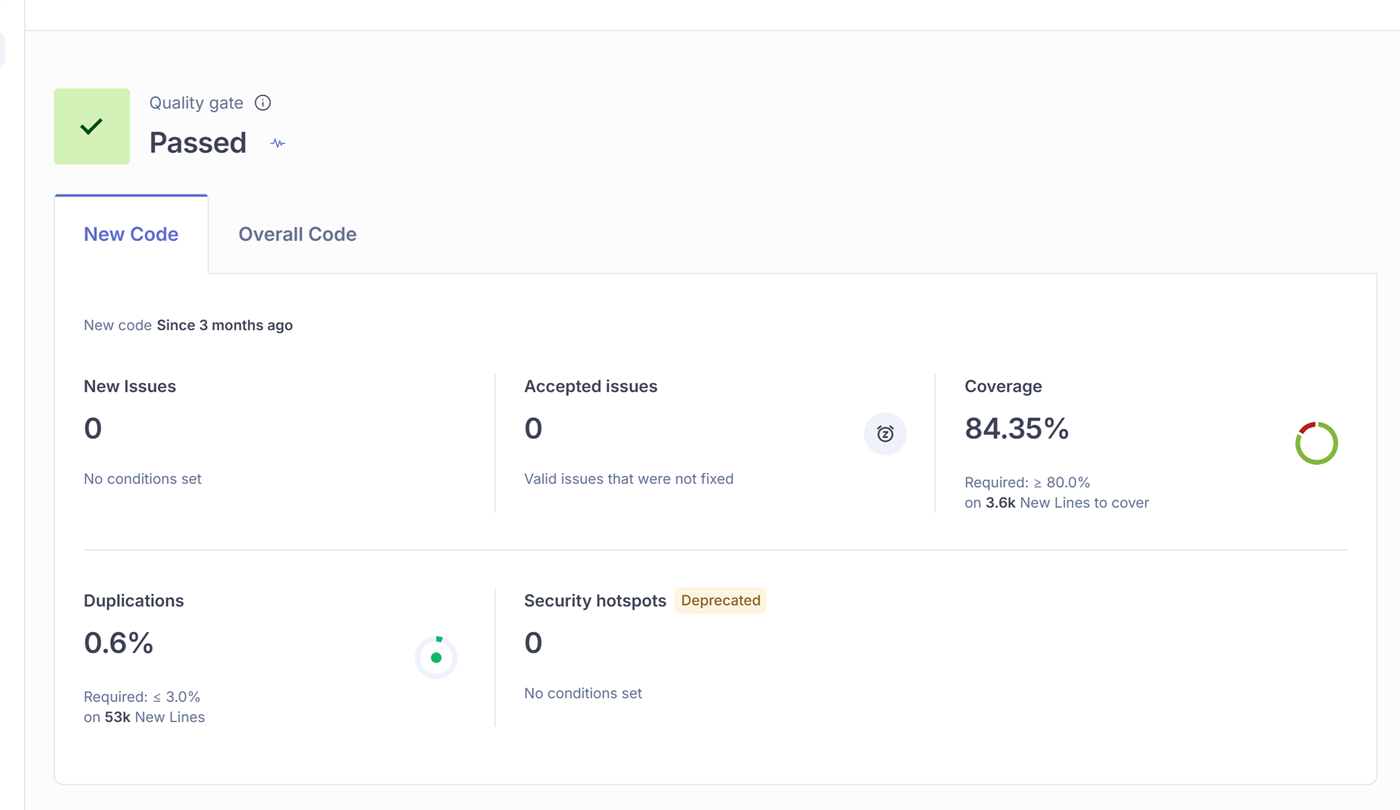
\includegraphics[width=0.92\textwidth,height=0.72\textheight,keepaspectratio]{figures/captures/annexe-sonarcloud.png}
    \caption{Porte de qualité, anomalies et couverture du code dans SonarCloud}
    \label{fig:annexe-sonarcloud}
\end{figure}

La valeur affichée pour la couverture (84,35 %) dépasse le seuil de 80 % appliqué au nouveau code. Les duplications restent sous la limite de 3 %. Ces indicateurs portent sur les modifications récentes et non sur l'ensemble du dépôt, ce qui correspond à l'objectif d'une analyse de régression : empêcher qu'une modification dégrade progressivement la qualité du code livré.

\subsection*{A.2 Supervision des services avec Grafana}
\addcontentsline{toc}{subsection}{A.2 Supervision des services avec Grafana}

Le tableau de bord Grafana interroge Prometheus, qui collecte les métriques exposées par le backend. Il présente l'état du service, le volume de requêtes par méthode et par statut, les erreurs, le temps de réponse, les routes les plus sollicitées et les indicateurs métier (ordres de travail ouverts, temps d'arrêt machine, interventions terminées, pièces en stock faible).

\begin{figure}[H]
    \centering
    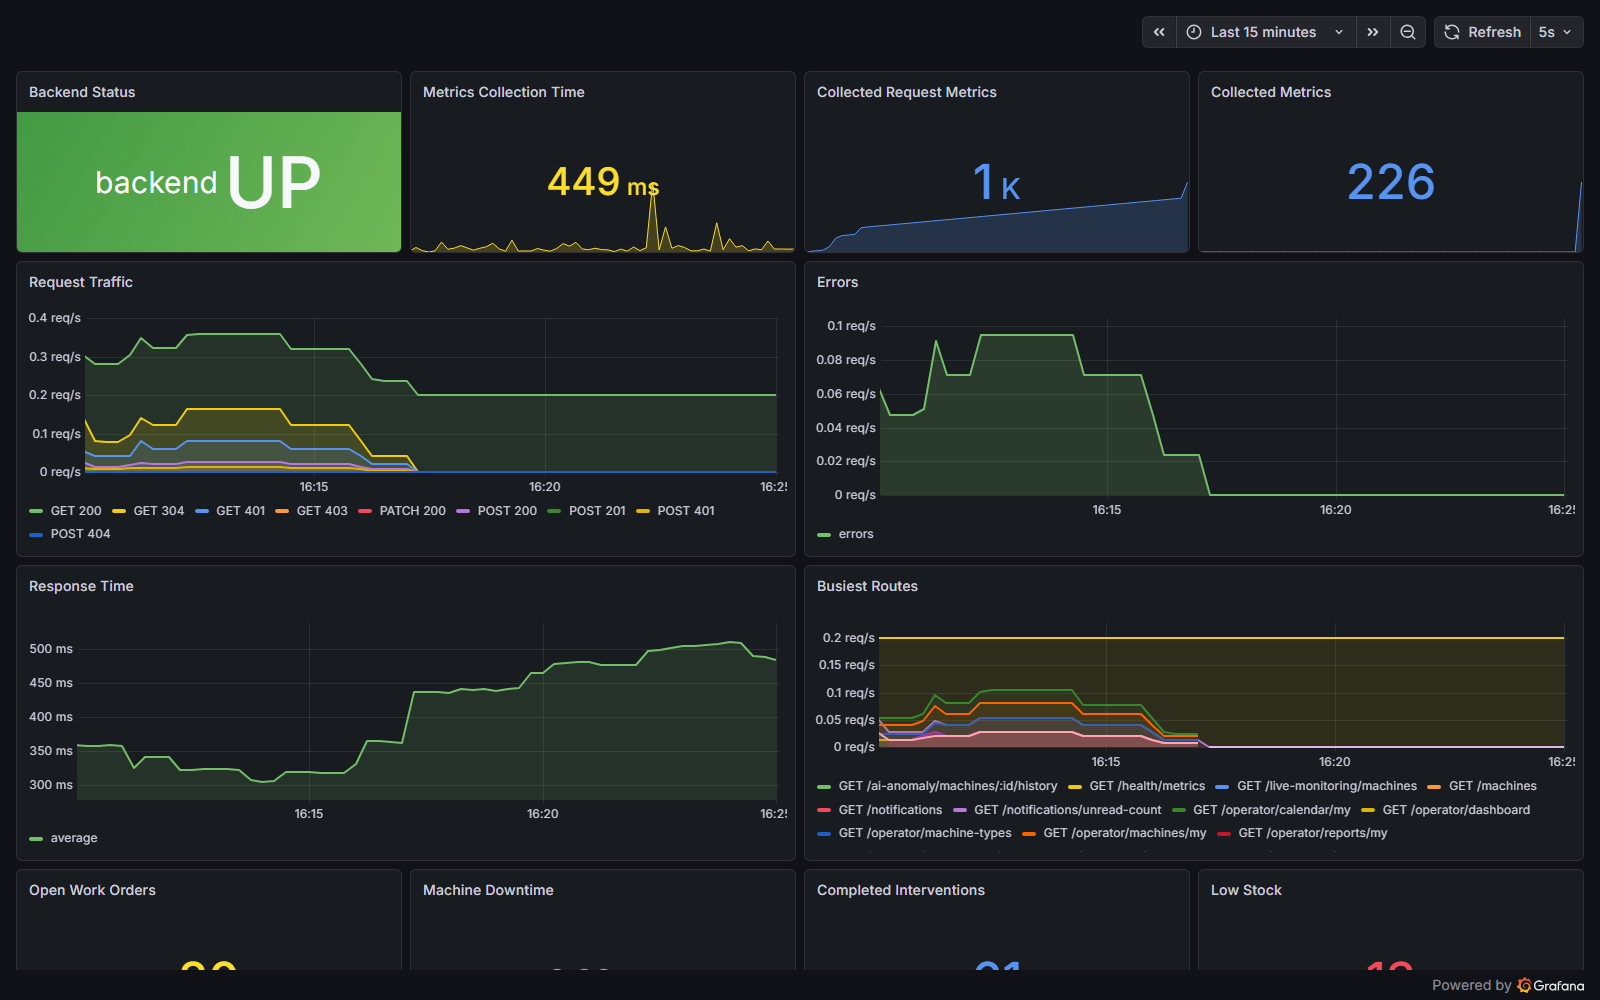
\includegraphics[width=0.95\textwidth,height=0.72\textheight,keepaspectratio]{figures/captures/annexe-grafana.png}
    \caption{Supervision des services : trafic, temps de réponse, erreurs et indicateurs métier}
    \label{fig:annexe-grafana}
\end{figure}

Les panneaux de trafic et de latence sont alimentés uniquement lorsque l'application reçoit des requêtes : une période d'inactivité produit des courbes plates sans que le service soit pour autant indisponible. L'état du backend, la date de collecte et le nombre de métriques collectées permettent de distinguer une absence de trafic d'une absence de collecte. Les alertes décrites au Sprint 7 s'appuient sur ces mêmes séries : une collecte interrompue, un taux d'erreurs serveur élevé ou une latence moyenne dégradée déclenchent une alerte.
